% !TEX encoding = UTF-8 Unicode
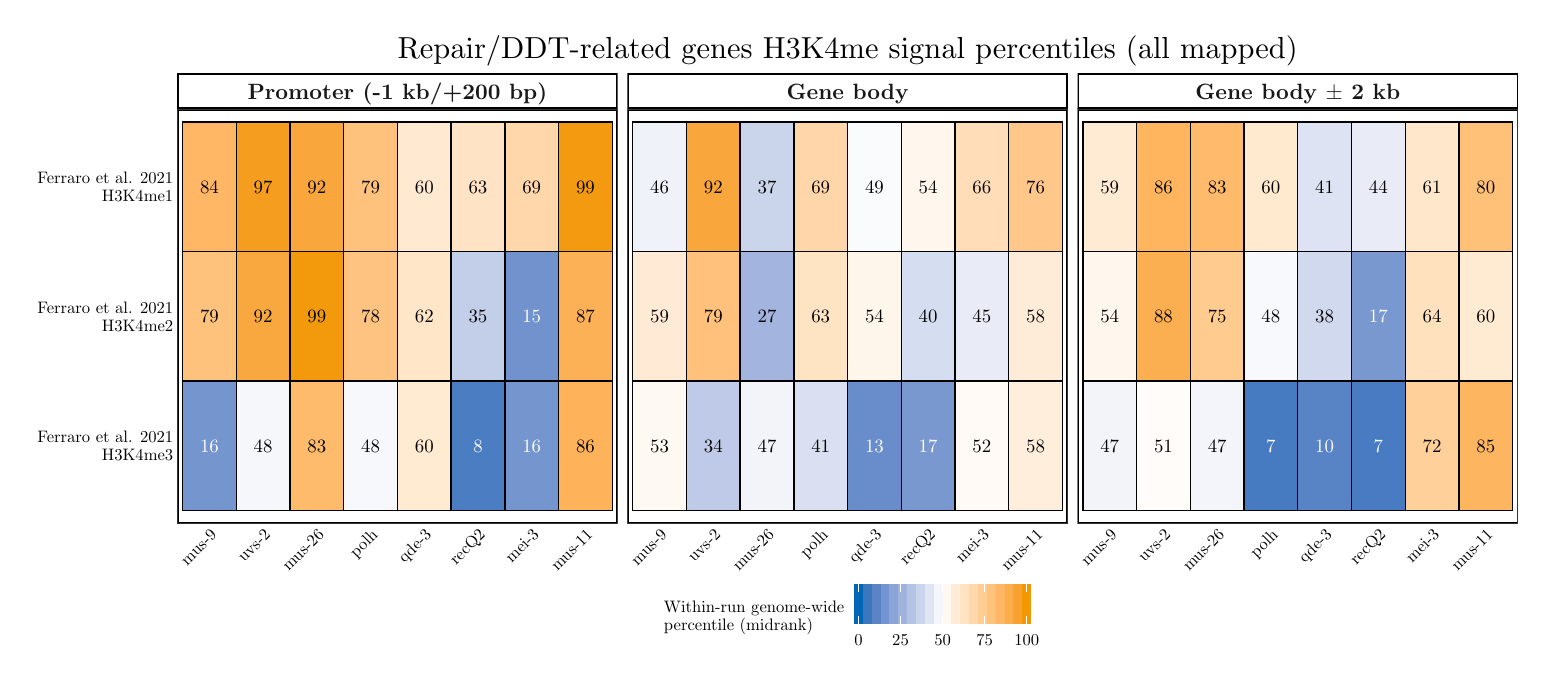
\begin{tikzpicture}[x=1pt,y=1pt]
\definecolor{fillColor}{RGB}{255,255,255}
\path[use as bounding box,fill=fillColor,fill opacity=0.00] (0,0) rectangle (542.02,231.26);
\begin{scope}
\path[clip] (  0.00,  0.00) rectangle (542.02,231.26);
\definecolor{drawColor}{RGB}{255,255,255}
\definecolor{fillColor}{RGB}{255,255,255}

\path[draw=drawColor,line width= 0.7pt,line join=round,line cap=round,fill=fillColor] ( -0.00,  0.00) rectangle (542.02,231.26);
\end{scope}
\begin{scope}
\path[clip] ( 54.02, 52.00) rectangle (213.19,201.87);
\definecolor{drawColor}{RGB}{0,0,0}
\definecolor{fillColor}{RGB}{255,255,255}

\path[draw=drawColor,line width= 1.1pt,line join=round,line cap=round,fill=fillColor] ( 54.02, 52.00) rectangle (213.19,201.87);
\definecolor{fillColor}{RGB}{255,183,101}

\path[draw=drawColor,line width= 0.5pt,fill=fillColor] ( 55.96,150.36) rectangle ( 75.37,197.19);
\definecolor{fillColor}{RGB}{245,157,30}

\path[draw=drawColor,line width= 0.5pt,fill=fillColor] ( 75.37,150.36) rectangle ( 94.78,197.19);
\definecolor{fillColor}{RGB}{249,167,61}

\path[draw=drawColor,line width= 0.5pt,fill=fillColor] ( 94.78,150.36) rectangle (114.19,197.19);
\definecolor{fillColor}{RGB}{255,194,125}

\path[draw=drawColor,line width= 0.5pt,fill=fillColor] (114.19,150.36) rectangle (133.61,197.19);
\definecolor{fillColor}{RGB}{255,233,209}

\path[draw=drawColor,line width= 0.5pt,fill=fillColor] (133.61,150.36) rectangle (153.02,197.19);
\definecolor{fillColor}{RGB}{255,227,196}

\path[draw=drawColor,line width= 0.5pt,fill=fillColor] (153.02,150.36) rectangle (172.43,197.19);
\definecolor{fillColor}{RGB}{255,215,170}

\path[draw=drawColor,line width= 0.5pt,fill=fillColor] (172.43,150.36) rectangle (191.84,197.19);
\definecolor{fillColor}{RGB}{243,154,17}

\path[draw=drawColor,line width= 0.5pt,fill=fillColor] (191.84,150.36) rectangle (211.25,197.19);
\definecolor{fillColor}{RGB}{255,194,124}

\path[draw=drawColor,line width= 0.5pt,fill=fillColor] ( 55.96,103.52) rectangle ( 75.37,150.36);
\definecolor{fillColor}{RGB}{249,168,64}

\path[draw=drawColor,line width= 0.5pt,fill=fillColor] ( 75.37,103.52) rectangle ( 94.78,150.36);
\definecolor{fillColor}{RGB}{243,154,12}

\path[draw=drawColor,line width= 0.5pt,fill=fillColor] ( 94.78,103.52) rectangle (114.19,150.36);
\definecolor{fillColor}{RGB}{255,195,129}

\path[draw=drawColor,line width= 0.5pt,fill=fillColor] (114.19,103.52) rectangle (133.61,150.36);
\definecolor{fillColor}{RGB}{255,230,201}

\path[draw=drawColor,line width= 0.5pt,fill=fillColor] (133.61,103.52) rectangle (153.02,150.36);
\definecolor{fillColor}{RGB}{195,206,233}

\path[draw=drawColor,line width= 0.5pt,fill=fillColor] (153.02,103.52) rectangle (172.43,150.36);
\definecolor{fillColor}{RGB}{113,146,205}

\path[draw=drawColor,line width= 0.5pt,fill=fillColor] (172.43,103.52) rectangle (191.84,150.36);
\definecolor{fillColor}{RGB}{253,177,87}

\path[draw=drawColor,line width= 0.5pt,fill=fillColor] (191.84,103.52) rectangle (211.25,150.36);
\definecolor{fillColor}{RGB}{116,149,206}

\path[draw=drawColor,line width= 0.5pt,fill=fillColor] ( 55.96, 56.68) rectangle ( 75.37,103.52);
\definecolor{fillColor}{RGB}{246,247,251}

\path[draw=drawColor,line width= 0.5pt,fill=fillColor] ( 75.37, 56.68) rectangle ( 94.78,103.52);
\definecolor{fillColor}{RGB}{255,187,108}

\path[draw=drawColor,line width= 0.5pt,fill=fillColor] ( 94.78, 56.68) rectangle (114.19,103.52);
\definecolor{fillColor}{RGB}{247,248,251}

\path[draw=drawColor,line width= 0.5pt,fill=fillColor] (114.19, 56.68) rectangle (133.61,103.52);
\definecolor{fillColor}{RGB}{255,234,210}

\path[draw=drawColor,line width= 0.5pt,fill=fillColor] (133.61, 56.68) rectangle (153.02,103.52);
\definecolor{fillColor}{RGB}{75,125,194}

\path[draw=drawColor,line width= 0.5pt,fill=fillColor] (153.02, 56.68) rectangle (172.43,103.52);
\definecolor{fillColor}{RGB}{117,149,206}

\path[draw=drawColor,line width= 0.5pt,fill=fillColor] (172.43, 56.68) rectangle (191.84,103.52);
\definecolor{fillColor}{RGB}{254,179,91}

\path[draw=drawColor,line width= 0.5pt,fill=fillColor] (191.84, 56.68) rectangle (211.25,103.52);

\node[text=drawColor,anchor=base,inner sep=0pt, outer sep=0pt, scale=  0.68] at ( 65.67,171.42) {84};

\node[text=drawColor,anchor=base,inner sep=0pt, outer sep=0pt, scale=  0.68] at ( 85.08,171.42) {97};

\node[text=drawColor,anchor=base,inner sep=0pt, outer sep=0pt, scale=  0.68] at (104.49,171.42) {92};

\node[text=drawColor,anchor=base,inner sep=0pt, outer sep=0pt, scale=  0.68] at (123.90,171.42) {79};

\node[text=drawColor,anchor=base,inner sep=0pt, outer sep=0pt, scale=  0.68] at (143.31,171.42) {60};

\node[text=drawColor,anchor=base,inner sep=0pt, outer sep=0pt, scale=  0.68] at (162.72,171.42) {63};

\node[text=drawColor,anchor=base,inner sep=0pt, outer sep=0pt, scale=  0.68] at (182.13,171.42) {69};

\node[text=drawColor,anchor=base,inner sep=0pt, outer sep=0pt, scale=  0.68] at (201.54,171.42) {99};

\node[text=drawColor,anchor=base,inner sep=0pt, outer sep=0pt, scale=  0.68] at ( 65.67,124.59) {79};

\node[text=drawColor,anchor=base,inner sep=0pt, outer sep=0pt, scale=  0.68] at ( 85.08,124.59) {92};

\node[text=drawColor,anchor=base,inner sep=0pt, outer sep=0pt, scale=  0.68] at (104.49,124.59) {99};

\node[text=drawColor,anchor=base,inner sep=0pt, outer sep=0pt, scale=  0.68] at (123.90,124.59) {78};

\node[text=drawColor,anchor=base,inner sep=0pt, outer sep=0pt, scale=  0.68] at (143.31,124.59) {62};

\node[text=drawColor,anchor=base,inner sep=0pt, outer sep=0pt, scale=  0.68] at (162.72,124.59) {35};
\definecolor{drawColor}{RGB}{255,255,255}

\node[text=drawColor,anchor=base,inner sep=0pt, outer sep=0pt, scale=  0.68] at (182.13,124.59) {15};
\definecolor{drawColor}{RGB}{0,0,0}

\node[text=drawColor,anchor=base,inner sep=0pt, outer sep=0pt, scale=  0.68] at (201.54,124.59) {87};
\definecolor{drawColor}{RGB}{255,255,255}

\node[text=drawColor,anchor=base,inner sep=0pt, outer sep=0pt, scale=  0.68] at ( 65.67, 77.75) {16};
\definecolor{drawColor}{RGB}{0,0,0}

\node[text=drawColor,anchor=base,inner sep=0pt, outer sep=0pt, scale=  0.68] at ( 85.08, 77.75) {48};

\node[text=drawColor,anchor=base,inner sep=0pt, outer sep=0pt, scale=  0.68] at (104.49, 77.75) {83};

\node[text=drawColor,anchor=base,inner sep=0pt, outer sep=0pt, scale=  0.68] at (123.90, 77.75) {48};

\node[text=drawColor,anchor=base,inner sep=0pt, outer sep=0pt, scale=  0.68] at (143.31, 77.75) {60};
\definecolor{drawColor}{RGB}{255,255,255}

\node[text=drawColor,anchor=base,inner sep=0pt, outer sep=0pt, scale=  0.68] at (162.72, 77.75) {8};

\node[text=drawColor,anchor=base,inner sep=0pt, outer sep=0pt, scale=  0.68] at (182.13, 77.75) {16};
\definecolor{drawColor}{RGB}{0,0,0}

\node[text=drawColor,anchor=base,inner sep=0pt, outer sep=0pt, scale=  0.68] at (201.54, 77.75) {86};
\definecolor{drawColor}{gray}{0.20}

\path[draw=drawColor,line width= 0.7pt,line join=round,line cap=round] ( 54.02, 52.00) rectangle (213.19,201.87);
\end{scope}
\begin{scope}
\path[clip] (216.69, 52.00) rectangle (375.86,201.87);
\definecolor{drawColor}{RGB}{0,0,0}
\definecolor{fillColor}{RGB}{255,255,255}

\path[draw=drawColor,line width= 1.1pt,line join=round,line cap=round,fill=fillColor] (216.69, 52.00) rectangle (375.86,201.87);
\definecolor{fillColor}{RGB}{239,242,249}

\path[draw=drawColor,line width= 0.5pt,fill=fillColor] (218.63,150.36) rectangle (238.04,197.19);
\definecolor{fillColor}{RGB}{249,167,60}

\path[draw=drawColor,line width= 0.5pt,fill=fillColor] (238.04,150.36) rectangle (257.45,197.19);
\definecolor{fillColor}{RGB}{202,213,236}

\path[draw=drawColor,line width= 0.5pt,fill=fillColor] (257.45,150.36) rectangle (276.86,197.19);
\definecolor{fillColor}{RGB}{255,214,169}

\path[draw=drawColor,line width= 0.5pt,fill=fillColor] (276.86,150.36) rectangle (296.27,197.19);
\definecolor{fillColor}{RGB}{250,251,253}

\path[draw=drawColor,line width= 0.5pt,fill=fillColor] (296.27,150.36) rectangle (315.68,197.19);
\definecolor{fillColor}{RGB}{255,247,237}

\path[draw=drawColor,line width= 0.5pt,fill=fillColor] (315.68,150.36) rectangle (335.09,197.19);
\definecolor{fillColor}{RGB}{255,221,185}

\path[draw=drawColor,line width= 0.5pt,fill=fillColor] (335.09,150.36) rectangle (354.51,197.19);
\definecolor{fillColor}{RGB}{255,199,138}

\path[draw=drawColor,line width= 0.5pt,fill=fillColor] (354.51,150.36) rectangle (373.92,197.19);
\definecolor{fillColor}{RGB}{255,235,213}

\path[draw=drawColor,line width= 0.5pt,fill=fillColor] (218.63,103.52) rectangle (238.04,150.36);
\definecolor{fillColor}{RGB}{255,193,123}

\path[draw=drawColor,line width= 0.5pt,fill=fillColor] (238.04,103.52) rectangle (257.45,150.36);
\definecolor{fillColor}{RGB}{163,181,222}

\path[draw=drawColor,line width= 0.5pt,fill=fillColor] (257.45,103.52) rectangle (276.86,150.36);
\definecolor{fillColor}{RGB}{255,228,196}

\path[draw=drawColor,line width= 0.5pt,fill=fillColor] (276.86,103.52) rectangle (296.27,150.36);
\definecolor{fillColor}{RGB}{255,246,235}

\path[draw=drawColor,line width= 0.5pt,fill=fillColor] (296.27,103.52) rectangle (315.68,150.36);
\definecolor{fillColor}{RGB}{213,221,240}

\path[draw=drawColor,line width= 0.5pt,fill=fillColor] (315.68,103.52) rectangle (335.09,150.36);
\definecolor{fillColor}{RGB}{233,236,247}

\path[draw=drawColor,line width= 0.5pt,fill=fillColor] (335.09,103.52) rectangle (354.51,150.36);
\definecolor{fillColor}{RGB}{255,236,216}

\path[draw=drawColor,line width= 0.5pt,fill=fillColor] (354.51,103.52) rectangle (373.92,150.36);
\definecolor{fillColor}{RGB}{255,249,243}

\path[draw=drawColor,line width= 0.5pt,fill=fillColor] (218.63, 56.68) rectangle (238.04,103.52);
\definecolor{fillColor}{RGB}{190,202,231}

\path[draw=drawColor,line width= 0.5pt,fill=fillColor] (238.04, 56.68) rectangle (257.45,103.52);
\definecolor{fillColor}{RGB}{243,244,250}

\path[draw=drawColor,line width= 0.5pt,fill=fillColor] (257.45, 56.68) rectangle (276.86,103.52);
\definecolor{fillColor}{RGB}{218,224,241}

\path[draw=drawColor,line width= 0.5pt,fill=fillColor] (276.86, 56.68) rectangle (296.27,103.52);
\definecolor{fillColor}{RGB}{104,141,202}

\path[draw=drawColor,line width= 0.5pt,fill=fillColor] (296.27, 56.68) rectangle (315.68,103.52);
\definecolor{fillColor}{RGB}{121,152,208}

\path[draw=drawColor,line width= 0.5pt,fill=fillColor] (315.68, 56.68) rectangle (335.09,103.52);
\definecolor{fillColor}{RGB}{255,250,246}

\path[draw=drawColor,line width= 0.5pt,fill=fillColor] (335.09, 56.68) rectangle (354.51,103.52);
\definecolor{fillColor}{RGB}{255,238,219}

\path[draw=drawColor,line width= 0.5pt,fill=fillColor] (354.51, 56.68) rectangle (373.92,103.52);

\node[text=drawColor,anchor=base,inner sep=0pt, outer sep=0pt, scale=  0.68] at (228.34,171.42) {46};

\node[text=drawColor,anchor=base,inner sep=0pt, outer sep=0pt, scale=  0.68] at (247.75,171.42) {92};

\node[text=drawColor,anchor=base,inner sep=0pt, outer sep=0pt, scale=  0.68] at (267.16,171.42) {37};

\node[text=drawColor,anchor=base,inner sep=0pt, outer sep=0pt, scale=  0.68] at (286.57,171.42) {69};

\node[text=drawColor,anchor=base,inner sep=0pt, outer sep=0pt, scale=  0.68] at (305.98,171.42) {49};

\node[text=drawColor,anchor=base,inner sep=0pt, outer sep=0pt, scale=  0.68] at (325.39,171.42) {54};

\node[text=drawColor,anchor=base,inner sep=0pt, outer sep=0pt, scale=  0.68] at (344.80,171.42) {66};

\node[text=drawColor,anchor=base,inner sep=0pt, outer sep=0pt, scale=  0.68] at (364.21,171.42) {76};

\node[text=drawColor,anchor=base,inner sep=0pt, outer sep=0pt, scale=  0.68] at (228.34,124.59) {59};

\node[text=drawColor,anchor=base,inner sep=0pt, outer sep=0pt, scale=  0.68] at (247.75,124.59) {79};

\node[text=drawColor,anchor=base,inner sep=0pt, outer sep=0pt, scale=  0.68] at (267.16,124.59) {27};

\node[text=drawColor,anchor=base,inner sep=0pt, outer sep=0pt, scale=  0.68] at (286.57,124.59) {63};

\node[text=drawColor,anchor=base,inner sep=0pt, outer sep=0pt, scale=  0.68] at (305.98,124.59) {54};

\node[text=drawColor,anchor=base,inner sep=0pt, outer sep=0pt, scale=  0.68] at (325.39,124.59) {40};

\node[text=drawColor,anchor=base,inner sep=0pt, outer sep=0pt, scale=  0.68] at (344.80,124.59) {45};

\node[text=drawColor,anchor=base,inner sep=0pt, outer sep=0pt, scale=  0.68] at (364.21,124.59) {58};

\node[text=drawColor,anchor=base,inner sep=0pt, outer sep=0pt, scale=  0.68] at (228.34, 77.75) {53};

\node[text=drawColor,anchor=base,inner sep=0pt, outer sep=0pt, scale=  0.68] at (247.75, 77.75) {34};

\node[text=drawColor,anchor=base,inner sep=0pt, outer sep=0pt, scale=  0.68] at (267.16, 77.75) {47};

\node[text=drawColor,anchor=base,inner sep=0pt, outer sep=0pt, scale=  0.68] at (286.57, 77.75) {41};
\definecolor{drawColor}{RGB}{255,255,255}

\node[text=drawColor,anchor=base,inner sep=0pt, outer sep=0pt, scale=  0.68] at (305.98, 77.75) {13};

\node[text=drawColor,anchor=base,inner sep=0pt, outer sep=0pt, scale=  0.68] at (325.39, 77.75) {17};
\definecolor{drawColor}{RGB}{0,0,0}

\node[text=drawColor,anchor=base,inner sep=0pt, outer sep=0pt, scale=  0.68] at (344.80, 77.75) {52};

\node[text=drawColor,anchor=base,inner sep=0pt, outer sep=0pt, scale=  0.68] at (364.21, 77.75) {58};
\definecolor{drawColor}{gray}{0.20}

\path[draw=drawColor,line width= 0.7pt,line join=round,line cap=round] (216.69, 52.00) rectangle (375.86,201.87);
\end{scope}
\begin{scope}
\path[clip] (379.36, 52.00) rectangle (538.52,201.87);
\definecolor{drawColor}{RGB}{0,0,0}
\definecolor{fillColor}{RGB}{255,255,255}

\path[draw=drawColor,line width= 1.1pt,line join=round,line cap=round,fill=fillColor] (379.36, 52.00) rectangle (538.53,201.87);
\definecolor{fillColor}{RGB}{255,235,212}

\path[draw=drawColor,line width= 0.5pt,fill=fillColor] (381.30,150.36) rectangle (400.71,197.19);
\definecolor{fillColor}{RGB}{254,181,94}

\path[draw=drawColor,line width= 0.5pt,fill=fillColor] (400.71,150.36) rectangle (420.12,197.19);
\definecolor{fillColor}{RGB}{255,186,107}

\path[draw=drawColor,line width= 0.5pt,fill=fillColor] (420.12,150.36) rectangle (439.53,197.19);
\definecolor{fillColor}{RGB}{255,233,207}

\path[draw=drawColor,line width= 0.5pt,fill=fillColor] (439.53,150.36) rectangle (458.94,197.19);
\definecolor{fillColor}{RGB}{221,227,242}

\path[draw=drawColor,line width= 0.5pt,fill=fillColor] (458.94,150.36) rectangle (478.35,197.19);
\definecolor{fillColor}{RGB}{233,236,247}

\path[draw=drawColor,line width= 0.5pt,fill=fillColor] (478.35,150.36) rectangle (497.76,197.19);
\definecolor{fillColor}{RGB}{255,231,204}

\path[draw=drawColor,line width= 0.5pt,fill=fillColor] (497.76,150.36) rectangle (517.17,197.19);
\definecolor{fillColor}{RGB}{255,192,120}

\path[draw=drawColor,line width= 0.5pt,fill=fillColor] (517.17,150.36) rectangle (536.58,197.19);
\definecolor{fillColor}{RGB}{255,247,237}

\path[draw=drawColor,line width= 0.5pt,fill=fillColor] (381.30,103.52) rectangle (400.71,150.36);
\definecolor{fillColor}{RGB}{252,175,81}

\path[draw=drawColor,line width= 0.5pt,fill=fillColor] (400.71,103.52) rectangle (420.12,150.36);
\definecolor{fillColor}{RGB}{255,203,143}

\path[draw=drawColor,line width= 0.5pt,fill=fillColor] (420.12,103.52) rectangle (439.53,150.36);
\definecolor{fillColor}{RGB}{248,249,252}

\path[draw=drawColor,line width= 0.5pt,fill=fillColor] (439.53,103.52) rectangle (458.94,150.36);
\definecolor{fillColor}{RGB}{208,217,238}

\path[draw=drawColor,line width= 0.5pt,fill=fillColor] (458.94,103.52) rectangle (478.35,150.36);
\definecolor{fillColor}{RGB}{121,152,208}

\path[draw=drawColor,line width= 0.5pt,fill=fillColor] (478.35,103.52) rectangle (497.76,150.36);
\definecolor{fillColor}{RGB}{255,225,190}

\path[draw=drawColor,line width= 0.5pt,fill=fillColor] (497.76,103.52) rectangle (517.17,150.36);
\definecolor{fillColor}{RGB}{255,234,210}

\path[draw=drawColor,line width= 0.5pt,fill=fillColor] (517.17,103.52) rectangle (536.58,150.36);
\definecolor{fillColor}{RGB}{243,244,250}

\path[draw=drawColor,line width= 0.5pt,fill=fillColor] (381.30, 56.68) rectangle (400.71,103.52);
\definecolor{fillColor}{RGB}{255,252,250}

\path[draw=drawColor,line width= 0.5pt,fill=fillColor] (400.71, 56.68) rectangle (420.12,103.52);
\definecolor{fillColor}{RGB}{243,245,251}

\path[draw=drawColor,line width= 0.5pt,fill=fillColor] (420.12, 56.68) rectangle (439.53,103.52);
\definecolor{fillColor}{RGB}{70,123,193}

\path[draw=drawColor,line width= 0.5pt,fill=fillColor] (439.53, 56.68) rectangle (458.94,103.52);
\definecolor{fillColor}{RGB}{88,131,197}

\path[draw=drawColor,line width= 0.5pt,fill=fillColor] (458.94, 56.68) rectangle (478.35,103.52);
\definecolor{fillColor}{RGB}{72,123,193}

\path[draw=drawColor,line width= 0.5pt,fill=fillColor] (478.35, 56.68) rectangle (497.76,103.52);
\definecolor{fillColor}{RGB}{255,208,154}

\path[draw=drawColor,line width= 0.5pt,fill=fillColor] (497.76, 56.68) rectangle (517.17,103.52);
\definecolor{fillColor}{RGB}{254,181,96}

\path[draw=drawColor,line width= 0.5pt,fill=fillColor] (517.17, 56.68) rectangle (536.58,103.52);

\node[text=drawColor,anchor=base,inner sep=0pt, outer sep=0pt, scale=  0.68] at (391.00,171.42) {59};

\node[text=drawColor,anchor=base,inner sep=0pt, outer sep=0pt, scale=  0.68] at (410.41,171.42) {86};

\node[text=drawColor,anchor=base,inner sep=0pt, outer sep=0pt, scale=  0.68] at (429.83,171.42) {83};

\node[text=drawColor,anchor=base,inner sep=0pt, outer sep=0pt, scale=  0.68] at (449.24,171.42) {60};

\node[text=drawColor,anchor=base,inner sep=0pt, outer sep=0pt, scale=  0.68] at (468.65,171.42) {41};

\node[text=drawColor,anchor=base,inner sep=0pt, outer sep=0pt, scale=  0.68] at (488.06,171.42) {44};

\node[text=drawColor,anchor=base,inner sep=0pt, outer sep=0pt, scale=  0.68] at (507.47,171.42) {61};

\node[text=drawColor,anchor=base,inner sep=0pt, outer sep=0pt, scale=  0.68] at (526.88,171.42) {80};

\node[text=drawColor,anchor=base,inner sep=0pt, outer sep=0pt, scale=  0.68] at (391.00,124.59) {54};

\node[text=drawColor,anchor=base,inner sep=0pt, outer sep=0pt, scale=  0.68] at (410.41,124.59) {88};

\node[text=drawColor,anchor=base,inner sep=0pt, outer sep=0pt, scale=  0.68] at (429.83,124.59) {75};

\node[text=drawColor,anchor=base,inner sep=0pt, outer sep=0pt, scale=  0.68] at (449.24,124.59) {48};

\node[text=drawColor,anchor=base,inner sep=0pt, outer sep=0pt, scale=  0.68] at (468.65,124.59) {38};
\definecolor{drawColor}{RGB}{255,255,255}

\node[text=drawColor,anchor=base,inner sep=0pt, outer sep=0pt, scale=  0.68] at (488.06,124.59) {17};
\definecolor{drawColor}{RGB}{0,0,0}

\node[text=drawColor,anchor=base,inner sep=0pt, outer sep=0pt, scale=  0.68] at (507.47,124.59) {64};

\node[text=drawColor,anchor=base,inner sep=0pt, outer sep=0pt, scale=  0.68] at (526.88,124.59) {60};

\node[text=drawColor,anchor=base,inner sep=0pt, outer sep=0pt, scale=  0.68] at (391.00, 77.75) {47};

\node[text=drawColor,anchor=base,inner sep=0pt, outer sep=0pt, scale=  0.68] at (410.41, 77.75) {51};

\node[text=drawColor,anchor=base,inner sep=0pt, outer sep=0pt, scale=  0.68] at (429.83, 77.75) {47};
\definecolor{drawColor}{RGB}{255,255,255}

\node[text=drawColor,anchor=base,inner sep=0pt, outer sep=0pt, scale=  0.68] at (449.24, 77.75) {7};

\node[text=drawColor,anchor=base,inner sep=0pt, outer sep=0pt, scale=  0.68] at (468.65, 77.75) {10};

\node[text=drawColor,anchor=base,inner sep=0pt, outer sep=0pt, scale=  0.68] at (488.06, 77.75) {7};
\definecolor{drawColor}{RGB}{0,0,0}

\node[text=drawColor,anchor=base,inner sep=0pt, outer sep=0pt, scale=  0.68] at (507.47, 77.75) {72};

\node[text=drawColor,anchor=base,inner sep=0pt, outer sep=0pt, scale=  0.68] at (526.88, 77.75) {85};
\definecolor{drawColor}{gray}{0.20}

\path[draw=drawColor,line width= 0.7pt,line join=round,line cap=round] (379.36, 52.00) rectangle (538.53,201.87);
\end{scope}
\begin{scope}
\path[clip] ( 54.02,201.87) rectangle (213.19,214.55);
\definecolor{drawColor}{RGB}{0,0,0}
\definecolor{fillColor}{RGB}{255,255,255}

\path[draw=drawColor,line width= 1.1pt,line join=round,line cap=round,fill=fillColor] ( 54.02,201.87) rectangle (213.19,214.55);
\definecolor{drawColor}{gray}{0.10}

\node[text=drawColor,anchor=base,inner sep=0pt, outer sep=0pt, scale=  0.80] at (133.61,205.45) {\bfseries Promoter (-1 kb/+200 bp)};
\end{scope}
\begin{scope}
\path[clip] (216.69,201.87) rectangle (375.86,214.55);
\definecolor{drawColor}{RGB}{0,0,0}
\definecolor{fillColor}{RGB}{255,255,255}

\path[draw=drawColor,line width= 1.1pt,line join=round,line cap=round,fill=fillColor] (216.69,201.87) rectangle (375.86,214.55);
\definecolor{drawColor}{gray}{0.10}

\node[text=drawColor,anchor=base,inner sep=0pt, outer sep=0pt, scale=  0.80] at (296.27,205.45) {\bfseries Gene body};
\end{scope}
\begin{scope}
\path[clip] (379.36,201.87) rectangle (538.52,214.55);
\definecolor{drawColor}{RGB}{0,0,0}
\definecolor{fillColor}{RGB}{255,255,255}

\path[draw=drawColor,line width= 1.1pt,line join=round,line cap=round,fill=fillColor] (379.36,201.87) rectangle (538.53,214.55);
\definecolor{drawColor}{gray}{0.10}

\node[text=drawColor,anchor=base,inner sep=0pt, outer sep=0pt, scale=  0.80] at (458.94,205.45) {\bfseries Gene body $\pm$ 2 kb};
\end{scope}
\begin{scope}
\path[clip] (  0.00,  0.00) rectangle (542.02,231.26);
\definecolor{drawColor}{RGB}{0,0,0}

\node[text=drawColor,rotate= 45.00,anchor=base east,inner sep=0pt, outer sep=0pt, scale=  0.60] at ( 68.59, 47.68) {mus-9};

\node[text=drawColor,rotate= 45.00,anchor=base east,inner sep=0pt, outer sep=0pt, scale=  0.60] at ( 88.00, 47.68) {uvs-2};

\node[text=drawColor,rotate= 45.00,anchor=base east,inner sep=0pt, outer sep=0pt, scale=  0.60] at (107.41, 47.68) {mus-26};

\node[text=drawColor,rotate= 45.00,anchor=base east,inner sep=0pt, outer sep=0pt, scale=  0.60] at (126.82, 47.68) {polh};

\node[text=drawColor,rotate= 45.00,anchor=base east,inner sep=0pt, outer sep=0pt, scale=  0.60] at (146.23, 47.68) {qde-3};

\node[text=drawColor,rotate= 45.00,anchor=base east,inner sep=0pt, outer sep=0pt, scale=  0.60] at (165.64, 47.68) {recQ2};

\node[text=drawColor,rotate= 45.00,anchor=base east,inner sep=0pt, outer sep=0pt, scale=  0.60] at (185.05, 47.68) {mei-3};

\node[text=drawColor,rotate= 45.00,anchor=base east,inner sep=0pt, outer sep=0pt, scale=  0.60] at (204.47, 47.68) {mus-11};
\end{scope}
\begin{scope}
\path[clip] (  0.00,  0.00) rectangle (542.02,231.26);
\definecolor{drawColor}{RGB}{0,0,0}

\node[text=drawColor,rotate= 45.00,anchor=base east,inner sep=0pt, outer sep=0pt, scale=  0.60] at (231.26, 47.68) {mus-9};

\node[text=drawColor,rotate= 45.00,anchor=base east,inner sep=0pt, outer sep=0pt, scale=  0.60] at (250.67, 47.68) {uvs-2};

\node[text=drawColor,rotate= 45.00,anchor=base east,inner sep=0pt, outer sep=0pt, scale=  0.60] at (270.08, 47.68) {mus-26};

\node[text=drawColor,rotate= 45.00,anchor=base east,inner sep=0pt, outer sep=0pt, scale=  0.60] at (289.49, 47.68) {polh};

\node[text=drawColor,rotate= 45.00,anchor=base east,inner sep=0pt, outer sep=0pt, scale=  0.60] at (308.90, 47.68) {qde-3};

\node[text=drawColor,rotate= 45.00,anchor=base east,inner sep=0pt, outer sep=0pt, scale=  0.60] at (328.31, 47.68) {recQ2};

\node[text=drawColor,rotate= 45.00,anchor=base east,inner sep=0pt, outer sep=0pt, scale=  0.60] at (347.72, 47.68) {mei-3};

\node[text=drawColor,rotate= 45.00,anchor=base east,inner sep=0pt, outer sep=0pt, scale=  0.60] at (367.13, 47.68) {mus-11};
\end{scope}
\begin{scope}
\path[clip] (  0.00,  0.00) rectangle (542.02,231.26);
\definecolor{drawColor}{RGB}{0,0,0}

\node[text=drawColor,rotate= 45.00,anchor=base east,inner sep=0pt, outer sep=0pt, scale=  0.60] at (393.93, 47.68) {mus-9};

\node[text=drawColor,rotate= 45.00,anchor=base east,inner sep=0pt, outer sep=0pt, scale=  0.60] at (413.34, 47.68) {uvs-2};

\node[text=drawColor,rotate= 45.00,anchor=base east,inner sep=0pt, outer sep=0pt, scale=  0.60] at (432.75, 47.68) {mus-26};

\node[text=drawColor,rotate= 45.00,anchor=base east,inner sep=0pt, outer sep=0pt, scale=  0.60] at (452.16, 47.68) {polh};

\node[text=drawColor,rotate= 45.00,anchor=base east,inner sep=0pt, outer sep=0pt, scale=  0.60] at (471.57, 47.68) {qde-3};

\node[text=drawColor,rotate= 45.00,anchor=base east,inner sep=0pt, outer sep=0pt, scale=  0.60] at (490.98, 47.68) {recQ2};

\node[text=drawColor,rotate= 45.00,anchor=base east,inner sep=0pt, outer sep=0pt, scale=  0.60] at (510.39, 47.68) {mei-3};

\node[text=drawColor,rotate= 45.00,anchor=base east,inner sep=0pt, outer sep=0pt, scale=  0.60] at (529.80, 47.68) {mus-11};
\end{scope}
\begin{scope}
\path[clip] (  0.00,  0.00) rectangle (542.02,231.26);
\definecolor{drawColor}{RGB}{0,0,0}

\node[text=drawColor,anchor=base east,inner sep=0pt, outer sep=0pt, scale=  0.60] at ( 52.62, 81.28) {Ferraro et al. 2021};

\node[text=drawColor,anchor=base east,inner sep=0pt, outer sep=0pt, scale=  0.60] at ( 52.62, 74.80) {H3K4me3};

\node[text=drawColor,anchor=base east,inner sep=0pt, outer sep=0pt, scale=  0.60] at ( 52.62,128.11) {Ferraro et al. 2021};

\node[text=drawColor,anchor=base east,inner sep=0pt, outer sep=0pt, scale=  0.60] at ( 52.62,121.63) {H3K4me2};

\node[text=drawColor,anchor=base east,inner sep=0pt, outer sep=0pt, scale=  0.60] at ( 52.62,174.95) {Ferraro et al. 2021};

\node[text=drawColor,anchor=base east,inner sep=0pt, outer sep=0pt, scale=  0.60] at ( 52.62,168.47) {H3K4me1};
\end{scope}
\begin{scope}
\path[clip] (  0.00,  0.00) rectangle (542.02,231.26);
\definecolor{fillColor}{RGB}{255,255,255}

\path[fill=fillColor] (226.43,  3.50) rectangle (366.12, 33.75);
\end{scope}
\begin{scope}
\path[clip] (  0.00,  0.00) rectangle (542.02,231.26);
\definecolor{drawColor}{RGB}{0,0,0}

\node[text=drawColor,anchor=base west,inner sep=0pt, outer sep=0pt, scale=  0.60] at (229.93, 19.80) {Within-run genome-wide};

\node[text=drawColor,anchor=base west,inner sep=0pt, outer sep=0pt, scale=  0.60] at (229.93, 13.32) {percentile (midrank)};
\end{scope}
\begin{scope}
\path[clip] (  0.00,  0.00) rectangle (542.02,231.26);
\definecolor{fillColor}{RGB}{0,103,183}

\path[fill=fillColor] (298.60, 15.80) rectangle (301.80, 30.25);
\definecolor{fillColor}{RGB}{60,118,190}

\path[fill=fillColor] (301.80, 15.80) rectangle (305.00, 30.25);
\definecolor{fillColor}{RGB}{90,132,198}

\path[fill=fillColor] (305.00, 15.80) rectangle (308.20, 30.25);
\definecolor{fillColor}{RGB}{115,148,206}

\path[fill=fillColor] (308.20, 15.80) rectangle (311.40, 30.25);
\definecolor{fillColor}{RGB}{138,164,213}

\path[fill=fillColor] (311.40, 15.80) rectangle (314.60, 30.25);
\definecolor{fillColor}{RGB}{160,179,221}

\path[fill=fillColor] (314.60, 15.80) rectangle (317.80, 30.25);
\definecolor{fillColor}{RGB}{181,196,228}

\path[fill=fillColor] (317.80, 15.80) rectangle (321.00, 30.25);
\definecolor{fillColor}{RGB}{202,212,236}

\path[fill=fillColor] (321.00, 15.80) rectangle (324.21, 30.25);
\definecolor{fillColor}{RGB}{224,229,243}

\path[fill=fillColor] (324.21, 15.80) rectangle (327.41, 30.25);
\definecolor{fillColor}{RGB}{245,246,251}

\path[fill=fillColor] (327.41, 15.80) rectangle (330.61, 30.25);
\definecolor{fillColor}{RGB}{255,249,242}

\path[fill=fillColor] (330.61, 15.80) rectangle (333.81, 30.25);
\definecolor{fillColor}{RGB}{255,237,218}

\path[fill=fillColor] (333.81, 15.80) rectangle (337.01, 30.25);
\definecolor{fillColor}{RGB}{255,227,195}

\path[fill=fillColor] (337.01, 15.80) rectangle (340.21, 30.25);
\definecolor{fillColor}{RGB}{255,216,171}

\path[fill=fillColor] (340.21, 15.80) rectangle (343.41, 30.25);
\definecolor{fillColor}{RGB}{255,205,148}

\path[fill=fillColor] (343.41, 15.80) rectangle (346.61, 30.25);
\definecolor{fillColor}{RGB}{255,194,124}

\path[fill=fillColor] (346.61, 15.80) rectangle (349.81, 30.25);
\definecolor{fillColor}{RGB}{255,183,101}

\path[fill=fillColor] (349.81, 15.80) rectangle (353.01, 30.25);
\definecolor{fillColor}{RGB}{251,173,76}

\path[fill=fillColor] (353.01, 15.80) rectangle (356.21, 30.25);
\definecolor{fillColor}{RGB}{247,162,48}

\path[fill=fillColor] (356.21, 15.80) rectangle (359.42, 30.25);
\definecolor{fillColor}{RGB}{242,152,0}

\path[fill=fillColor] (359.42, 15.80) rectangle (362.62, 30.25);
\end{scope}
\begin{scope}
\path[clip] (  0.00,  0.00) rectangle (542.02,231.26);
\definecolor{drawColor}{RGB}{255,255,255}

\path[draw=drawColor,line width= 0.4pt,line join=round] (300.20, 18.69) --
	(300.20, 15.80);

\path[draw=drawColor,line width= 0.4pt,line join=round] (315.40, 18.69) --
	(315.40, 15.80);

\path[draw=drawColor,line width= 0.4pt,line join=round] (330.61, 18.69) --
	(330.61, 15.80);

\path[draw=drawColor,line width= 0.4pt,line join=round] (345.81, 18.69) --
	(345.81, 15.80);

\path[draw=drawColor,line width= 0.4pt,line join=round] (361.02, 18.69) --
	(361.02, 15.80);

\path[draw=drawColor,line width= 0.4pt,line join=round] (300.20, 27.36) --
	(300.20, 30.25);

\path[draw=drawColor,line width= 0.4pt,line join=round] (315.40, 27.36) --
	(315.40, 30.25);

\path[draw=drawColor,line width= 0.4pt,line join=round] (330.61, 27.36) --
	(330.61, 30.25);

\path[draw=drawColor,line width= 0.4pt,line join=round] (345.81, 27.36) --
	(345.81, 30.25);

\path[draw=drawColor,line width= 0.4pt,line join=round] (361.02, 27.36) --
	(361.02, 30.25);
\end{scope}
\begin{scope}
\path[clip] (  0.00,  0.00) rectangle (542.02,231.26);
\definecolor{drawColor}{RGB}{0,0,0}

\node[text=drawColor,anchor=base,inner sep=0pt, outer sep=0pt, scale=  0.60] at (300.20,  8.17) {0};

\node[text=drawColor,anchor=base,inner sep=0pt, outer sep=0pt, scale=  0.60] at (315.40,  8.17) {25};

\node[text=drawColor,anchor=base,inner sep=0pt, outer sep=0pt, scale=  0.60] at (330.61,  8.17) {50};

\node[text=drawColor,anchor=base,inner sep=0pt, outer sep=0pt, scale=  0.60] at (345.81,  8.17) {75};

\node[text=drawColor,anchor=base,inner sep=0pt, outer sep=0pt, scale=  0.60] at (361.02,  8.17) {100};
\end{scope}
\begin{scope}
\path[clip] (  0.00,  0.00) rectangle (542.02,231.26);
\definecolor{drawColor}{RGB}{0,0,0}

\node[text=drawColor,anchor=base,inner sep=0pt, outer sep=0pt, scale=  1.10] at (296.27,220.19) {Repair/DDT-related genes H3K4me signal percentiles (all mapped)};
\end{scope}
\end{tikzpicture}
